\begin{frame}{Contribution: Range Space}
    \begin{definition}{\textbf{A range space}}
    $\mathcal{R} \subseteq \mathcal{I}$ is a set of I-states, equipped with two
    operations:
    \end{definition}
    \begin{columns}
        \begin{column}{.5\textwidth}
          \begin{enumerate}
          \item \emph{Approximate action update function} $T: \mathcal{R} \times U \to
            \mathcal{R}$:
            $$\bigcup_{x_k \in \eta_k} F(x_k, u_k) \subseteq T(A(\eta_k), u_k)$$
          \item \emph{Approximate observation update function} $O: \mathcal{R} \times
            Y \to \mathcal{R}$:
            $$\eta_k \cap H(y_k) \subseteq O(A(\eta_k), u_k)$$
          \end{enumerate}
          \textcolor{scred}{Intuition: always over-approximate I-state:
            $\eta_k \subseteq A(\eta_k)$}
        \end{column}
        \begin{column}{.4\textwidth}
            \begin{figure}
    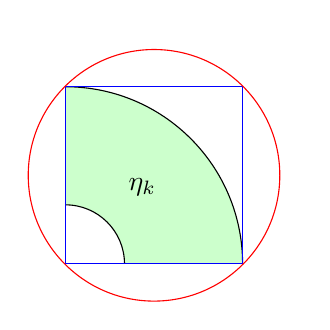
\begin{tikzpicture}[scale=0.75]
      \begin{scope}
        \clip (0,0) rectangle (4,4);
        \draw[fill=green!20] (0,0) circle (3cm);
        \draw[fill=white] (0,0) circle (1cm);  
      \end{scope}
      \draw[blue] (0,0) -- (3,0) -- (3,3) -- (0,3) -- (0,0);
      \draw[red]  (1.5,1.5) circle (2.13cm);
      \node at (1.3,1.3) {$\eta_k$};    
    \end{tikzpicture} 
    \caption{\scriptsize{An \emph{I-state} $\eta_k$ (shaded region),
        over-approximations $A(\eta_k)$ using disk (red circle) and rectangle
        (blue). }}
\end{figure}
        \end{column}
    \end{columns}
\end{frame}